\documentclass[aspectratio=169,12pt]{beamer}
\usepackage[portuguese]{babel}
\usepackage[utf8]{inputenc}
\usepackage{graphicx}
\usepackage{booktabs}
\usepackage{hyperref}
\usepackage{xcolor}
\usepackage{listings}
\usepackage[T1]{fontenc}
\usepackage{pmboxdraw}
\sloppy

\usetheme{Madrid}
\usecolortheme{seahorse}

\definecolor{codegray}{rgb}{0.5,0.5,0.5}
\definecolor{codeblue}{rgb}{0.13,0.13,1}
\definecolor{codegreen}{rgb}{0,0.6,0}
\definecolor{backcolour}{rgb}{0.96,0.96,0.98}

\lstdefinestyle{mystyle}{
    backgroundcolor=\color{backcolour},
    commentstyle=\color{codegreen},
    keywordstyle=\color{codeblue},
    numberstyle=\tiny\color{codegray},
    stringstyle=\color{magenta},
    basicstyle=\ttfamily\small,
    breakatwhitespace=false,
    breaklines=true,
    keepspaces=true,
    numbers=left,
    numbersep=5pt,
    showspaces=false,
    showstringspaces=false,
    showtabs=false,
    tabsize=2
}
\lstset{style=mystyle}

\title{Ferramenta de Segurança da Informação \\ Wazuh SIEM}
\author{Eduardo Marinho de Paiva \\ João Victor Amaral de Souza \\ Luiz Henrique Alves Ferreira \\ Marlos Emanuel da Silveira Fontes \\ Paulo Sérgio Silva de Medeiros \\ Vinícius Eduardo Freitas de Sales}
\institute{Universidade do Estado do Rio Grande do Norte \\ MDI 0209 -- Segurança de Sistemas}
\date{2026}

\begin{document}

\begin{frame}
\titlepage
\end{frame}

\begin{frame}{Ambiente do Laboratório --- Topologia}
\centering
\vspace{-0.3cm}
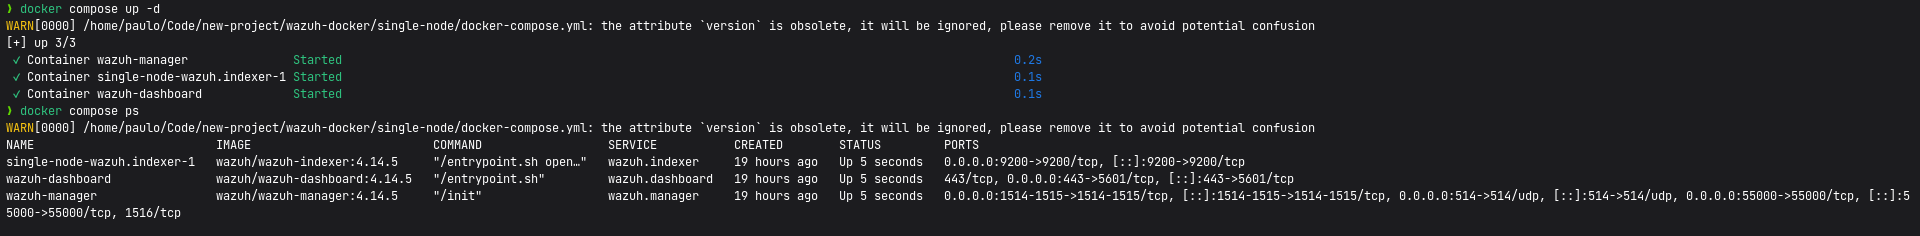
\includegraphics[width=0.9\textwidth]{docker-terminal.png}

\vspace{0.3cm}
\begin{tabular}{ll}
\toprule
\textbf{Máquina} & \textbf{Função} \\
\midrule
Kali Linux 2026 (VM) & Atacante --- nmap, hydra, curl \\
Arch Linux (Físico) & Servidor vítima + Wazuh Docker + DVWA \\
Wazuh Docker Stack & Manager, Indexer, Dashboard \\
\bottomrule
\end{tabular}
\end{frame}

\begin{frame}{Instalação}
\vspace{0.3cm}
\textbf{Processo:}
\begin{enumerate}
    \item Clone do \texttt{wazuh-docker} (branch 4.9.0)
    \item Ajuste do heap OpenSearch: \texttt{-Xms4g -Xmx4g} $\rightarrow$ \texttt{-Xms1g -Xmx1g}
    \item Geração de certificados SSL + \texttt{docker compose up -d}
    \item Instalação do agente Wazuh no Arch Linux
    \item Criação da VM Kali via VirtualBox
\end{enumerate}

\vspace{0.3cm}
\textbf{Problemas encontrados:}
\begin{itemize}
    \item OpenSearch com heap padrão de 4 GB impedia inicialização em 16 GB RAM
    \item Certificados SSL falharam na primeira execução (permissões)
    \item Pacote do agente Wazuh não disponível nos repositórios oficiais do Arch
\end{itemize}
\end{frame}

\begin{frame}{Configuração}
\vspace{0.3cm}
\textbf{28 regras customizadas de compliance:}
\begin{itemize}
    \item NIST CSF: 12 regras
    \item ISO 27001: 5 regras
    \item LGPD: 5 regras
    \item MITRE ATT\&CK: 4 regras
    \item Métricas: 2 regras
\end{itemize}

\vspace{0.3cm}
\textbf{Outras configurações:}
\begin{itemize}
    \item FIM em tempo real: \texttt{/etc/passwd}, \texttt{/etc/shadow}, \texttt{/data/clientes}
    \item Journal-bridge: logs do systemd $\rightarrow$ agente Wazuh
    \item Ajustes de segurança: nftables FORWARD accept, sshd sem penalidades
\end{itemize}
\end{frame}

\begin{frame}{Integração e Fluxo de Dados}
\centering
\vspace{0.3cm}
\textbf{Fluxo:}
\begin{enumerate}
    \item Kali gera ataques (nmap, hydra, curl, SSH) $\rightarrow$ Arch Host
    \item Wazuh Agent coleta logs (journal-bridge) e envia para o Manager (porta 1514)
    \item Manager decodifica e aplica regras de correlação
    \item Alertas indexados no OpenSearch e exibidos no Dashboard
\end{enumerate}

\vspace{0.3cm}
\textbf{Integrações:}
\begin{itemize}
    \item Journald $\rightarrow$ Wazuh Agent (via journal-bridge)
    \item Restic $\rightarrow$ Wazuh (syslog)
    \item Kali $\leftrightarrow$ Arch Host (rede Host-Only 192.168.56.0/24)
\end{itemize}
\end{frame}

\begin{frame}{Testes Funcionais}
\textbf{Teste 1: Força Bruta SSH}
\begin{itemize}
    \item Hydra com 15 senhas contra SSH do host
    \item 15 alertas SID 200003 (severidade 8)
    \item Com 100+ senhas: correlação SID 200040 (severidade 15)
\end{itemize}

\vspace{0.3cm}
\textbf{Teste 2: SQL Injection com Vazamento LGPD}
\begin{itemize}
    \item UNION SELECT na tabela \texttt{clientes.pessoas}
    \item Alerta SID 200031 (severidade 12)
    \item Classificação: MITRE T1190 + LGPD Art. 46/49
\end{itemize}

\vspace{0.3cm}
\centering
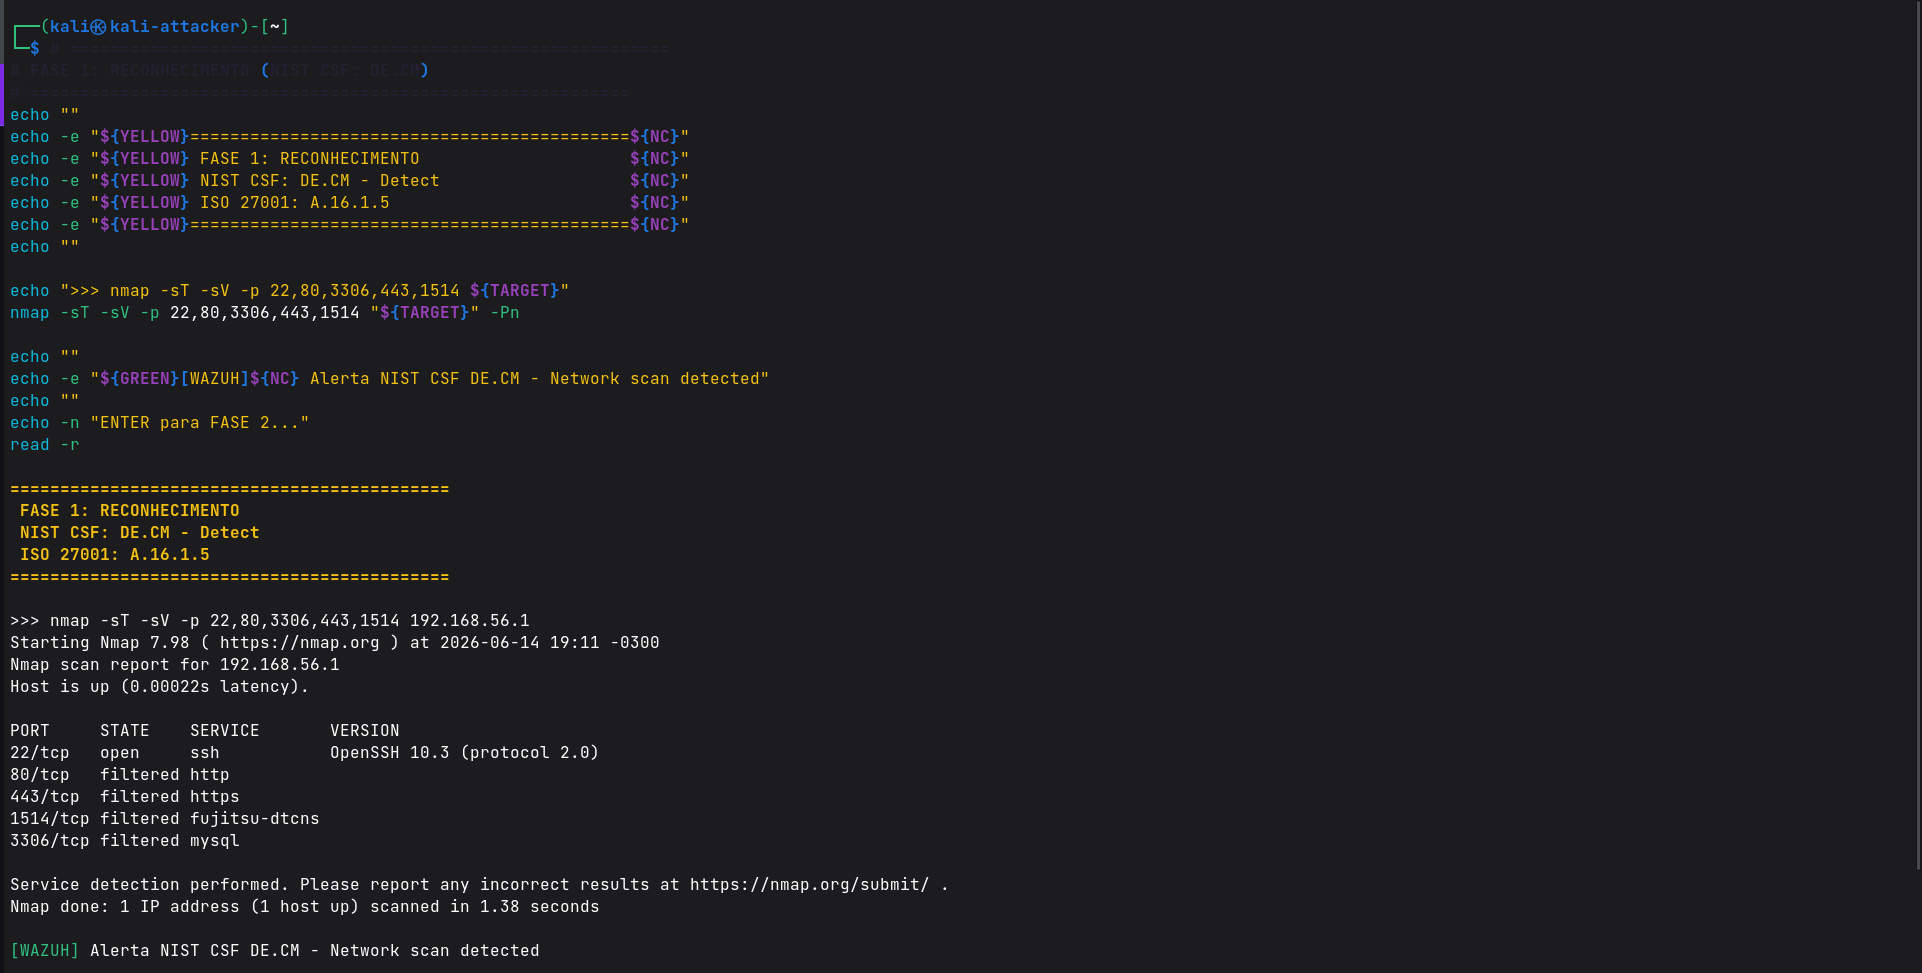
\includegraphics[width=0.7\textwidth]{ataques-brute.png}
\end{frame}

\begin{frame}{Evidências --- Dashboard}
\centering

\includegraphics[width=0.95\textwidth]{ataques-dashboard.png}
\end{frame}

\begin{frame}{Evidências --- SQL Injection e MITRE}
\centering

\includegraphics[width=0.85\textwidth]{sql-inje.png}

\vspace{0.5cm}
\centering

\includegraphics[width=0.85\textwidth]{dashboard-mitre.png}
\end{frame}

\begin{frame}{Alertas e Métricas}
\centering
\footnotesize
\begin{tabular}{lll}
\toprule
\textbf{SID} & \textbf{Descrição} & \textbf{Severidade} \\
\midrule
200006 & NIST CSF DE.CM --- SSH scan & 8 \\
200003 & NIST CSF PR.AC --- SSH failure & 8 \\
200040 & BRUTE FORCE --- 30+ falhas/5min & 15 \\
200031 & MITRE T1190 --- SQL Injection LGPD & 12 \\
200004 & NIST CSF PR.DS --- File integrity & 9 \\
200033 & NIST CSF RC.RP --- Restore & 5 \\
\bottomrule
\end{tabular}

\vspace{0.5cm}
\textbf{Métricas:}
\begin{itemize}
    \item 644 alertas de brute force
    \item 100 eventos FIM (ransomware simulado)
    \item RTO de 12 min 30 s
\end{itemize}
\end{frame}

\end{document}
